
Water, being ``at the centre of the planetary drama of the Anthropocene'', is essential not only for earth system processes but also in supporting development and human well-being~\cite{gleeson2020a,gleeson2020b}.
As an integral part of earth system governance, successful water governance requires a deep understanding of changes in the complex relationships between humans and water~\cite{ahlstrom2021,biermann2012,steffen2020}.
Human activities stemming from our reliance on water have profoundly modified the natural water cycle, resulting in rivers that are dominated by a hybrid of social and natural drivers~\cite{sivapalan2012,qin2014a,abbott2019}.
Facing transitions from natural to human-dominated regimes, many big river basins worldwide (which are hot spots of civilization and economic growth) are urgently in need of more effective water governance~\cite{best2019,dibaldassarre2019}.

Water governance encompasses the political, social, economic, and administrative systems that regulate water use and management, dictating ``who gets water, when and how''~\cite{lasswell2018,allan2001}.
In this context, the United Nations Development Programme (UNDP) suggests that water governance determines water usage across three core aspects: ``When and what water to use?'' (stress), ``How does water provide different services for human well-being?'' (purpose), and ``Who can use water equally and efficiently?'' (allocation)~\cite{mariajacobson2013}.
% 为充分考虑这些人类活动影响,做出有助于水治理实践的评估,以往的综合指标主要可分成两类:评估水系统与评估治理系统。
Research into index-based water governance assessment generally fall into two categories: those that focus on water systems, and those that concentrate on governance systems.
On one hand, studies on governance systems typically employ an qualitative assessment to demonstrate what practices influence water governance, e.g., the OECD framework~\cite{oecd2018a}.
For quantitative studies, due to the lack of comprehensive and detailed information on key components for water governance assessment, these studies often resort to proxy datasets of human activities to create simpler indices~\cite{varis2019,huggins2020}.
On the other hand, studies focusing on water systems utilize intuitive indices to encapsulate the outcomes of governance, like the most widely concerned -water stress has been far developed by incorporating human's regulation step by step.
Specifically, traditional water stress index only demands and supply~\cite{gleick1996}, water scarcity index by involving storage~\cite{damkjaer2017}, and the even more integrated SFV-index includes flexibility~\cite{qin2019}.
Despite their usefulness, these water stress indices tend not to provide a comprehensive characterization of water governance, as they overlook the social aspect of water usage, i.e., the purpose and allocation of water use.
As a solution, we propose an integrated water governance index (IWGI) that factors in regional water use allocations and sectoral water use purpose, thereby offering a more comprehensive quantification of governance outcomes.

The impetus for developing this new index lies in the evolving practices of water governance driven by a blend of social and natural influences.
Firstly, climate change impacts on current water yield, coupled with escalating demands from economic activities and the need for water storage development, intensify water stress~\cite{qin2019,wada2014,huang2021}.
Secondly, the purpose of water in serving human well-being is witnessing a shift in trade-offs. The balance between provisioning uses (such as drinking water and food production) and non-provisioning uses (like energy production) is tilting, reflecting changes in societal needs and values~\cite{liu2017,florke2018,jaeger2019}.
Thirdly, the allocation of water across a basin is not solely determined by regional socio-economic and environmental contexts but is also increasingly influenced by systematic regulations~\cite{schmandt2021,speed2013}.
As we transition towards a human-dominated regime, these three interlinked aspects -stress, purpose, and allocation, are undergoing substantial changes.
Assessing them separately could lead to systematic failures in water governance, highlighting the need for a more integrated approach in evaluating water governance practices.

A critical step in understanding the successes and failures of water governance is to identify the different regimes that underpin it~\cite{kjellen2015, grafton2013}.
Regimes of water governance, the general guidelines of governing practices, arise within linked human-water systems (based on management, institutions, and exploitation) to create local equilibria in social-ecological structures and functions~\cite{falkenmark2021,bressers2013,loch2020,pahl-wostl2007}.
For example, under a human-dominated regime, reservoirs make water stress easier to be alleviated because of flexibility; growing energy and industrial demands make water services purposes lopsided to non-provisioning sectors; conveyance systems make water allocation more planned (Figure~\ref{fig:framework}~A)
However, the lack of a comprehensive but straightforward approach to identifying changes in water governance regimes represents a challenge for efforts to enhance the sustainability of water resource use.
Filling this gap, which is the aim of this paper, is essential for the appropriate alignment of human and water systems.


\begin{figure*}[!ht]
	\centerline{
		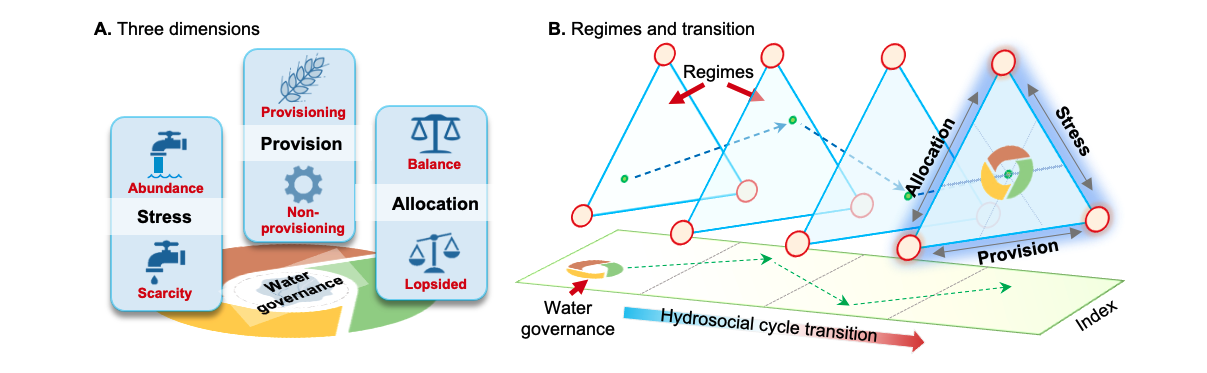
\includegraphics[width=1.1\linewidth]{main/framework.png}
	}
	\caption{
		\textbf{A.} Identifying the water governance regimes in transitions of a hydrosocial cycle with an integrated water governance index (IWGI). Water stress (S), purposes of water services (P), and water allocation (A) are three aspects to be considered.
		For example, reservoir construction (\ding{172} and \ding{173}) can relieve local water stress; The development of intensive irrigated agriculture (\ding{174}) and growth of energy industrial demand (\ding{175}) will change the purpose of water use; The water delivery system controls water allocation (\ding{176} and \ding{177}) within the basin system.
		\textbf{B.} Therefore, the methodology is to combine three aspects' corresponding indicators, and then an abrupt change of the IWGI can indicate a regime shift in water governance.
	}\label{fig:framework}
\end{figure*}


The Yellow River Basin (YRB), which contains the fifth-largest and most sediment-rich river in the world, needs integrated water governance because of geological and human history~\cite{mostern2021,best2019}.
Since the 1960s, governance practices such as reservoirs, levees, and conservation measures have contained the issues troubled by thousands of years of high sediment loads~\cite{wang2016a,song2020}.
However, new challenges such as decreased streamflows and water depletions occurred in more recent times, followed by different water governance practices like water use regulation and water transfer across basins~\cite{wang2019c}.
Today, it is still impossible to completely solve water stress, trade-offs between ecosystem services, or lopsided development in different regions in the YRB to the satisfaction of all actors~\cite{wohlfart2016}.
Governance challenges induced by environmental, economic, social, and political factors have resulted in YRB being among the most intensively-governed large river basins worldwide~\cite{nickum2021}.
Identifying regime shifts in water governance within the YRB can thus provide crucial insights into rapidly-changing big river basins and how governance may respond to meeting challenges to their sustainability.

% 这里我们整合了三个方向,提出了描绘流域人水关系的指数
Here, we depict three aspects of water governance -stress, purpose and allocation with corresponding indicators (see methods) and thus develop an Integrated Water Governance Index (IWGI) by equally weighting them, to indicate results from water governance (see Figure~\ref{fig:framework}~B).
% 使用案例研究
Then, by applying the index to a typical rapid-changing big river basin (the YRB), we show how IWGI helps detect and describe complicated water governance regimes comprehensively but straightforwardly.
Following synthetic analyses of the changes in water demand, supply, economic outcomes, and institutions, we interpret the leading causes of the regime shifts.
% 最后总结出一般性框架
Finally, we propose a general regime transition schema that offers a practical guideline for a coordinated approach to exploring the challenges faced by big river basin governance.
